\chapter{Đặc Tả Yêu Cầu Phần Mềm}

\section{Luồng màn hình và đặc tả}

\begin{figure}[htbp]
	\centering
	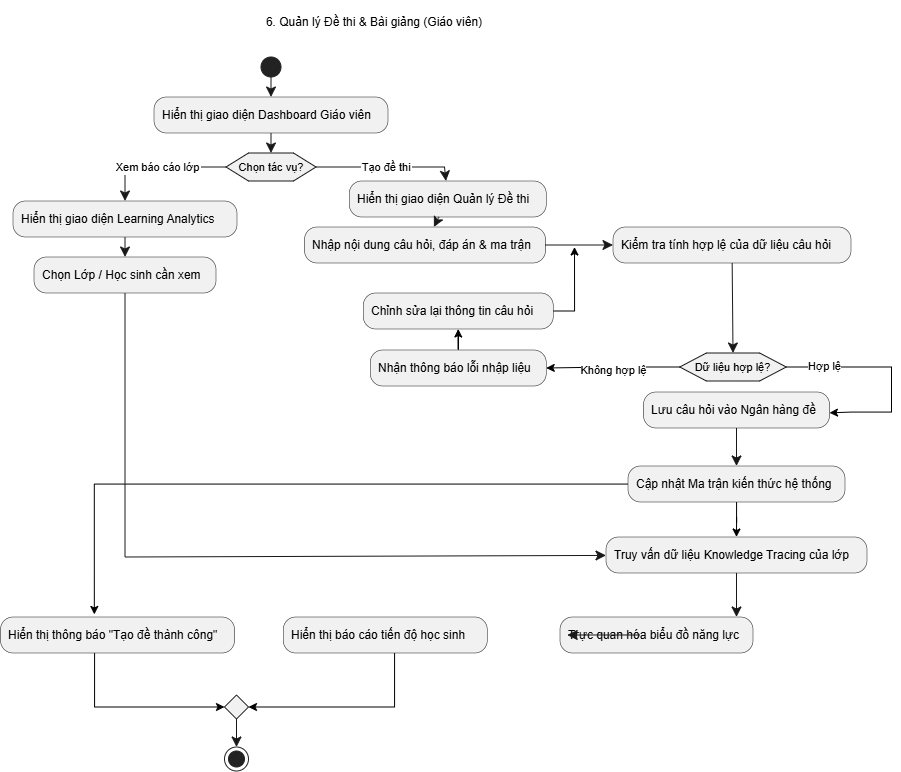
\includegraphics[width=0.85\textwidth]{Figures/Trang-2.drawio}
	\label{fig:luong_man_hinh_trang2}
\end{figure}

\clearpage % Lệnh ngắt trang tại đây để đẩy toàn bộ bảng sang trang 2

\renewcommand{\arraystretch}{1.25}
\begin{longtable}{|c|p{2.8cm}|p{4.2cm}|p{6.5cm}|}
	\hline
	\rowcolor{tableheader}
	\textbf{\#} & \textbf{Feature} & \textbf{Screen} & \textbf{Description} \\ \hline
	\endfirsthead
	1 & General & Trang chủ / Đăng nhập & Màn hình xác thực tài khoản dành riêng cho giáo viên/giảng viên. \\ \hline
	2 & Dashboard & Dashboard Giáo viên & Trang trung tâm hiển thị các lớp học đang đảm nhận, bài tập cần chấm và lịch dạy. \\ \hline
	3 & Class Management & Màn hình Quản lý Lớp học \& Danh sách Học viên & Quản lý thông tin chi tiết danh sách học sinh thuộc các lớp do giáo viên phụ trách. \\ \hline
	4 & Question Bank & Màn hình Ngân hàng Câu hỏi \& Đề thi & Kho lưu trữ, quản lý và phân loại các câu hỏi, ma trận đề thi theo chủ đề. \\ \hline
	5 & Test Creation & Màn hình Tạo mới / Cấu hình Đề thi \& Đáp án & Giao diện thiết lập đề thi mới, cài đặt đáp án, thang điểm và thời gian mở đề. \\ \hline
	6 & Assignment & Màn hình Phân công / Giao Bài tập cho Lớp & Giao diện chọn lớp nhận bài tập, đặt thời hạn nộp bài (deadline) và cài đặt thông báo. \\ \hline
	7 & Grading & Màn hình Quản lý Danh sách Bài nộp của Học sinh & Tổng hợp danh sách bài làm của học sinh theo trạng thái (Đã nộp, Chưa nộp, Cần chấm). \\ \hline
	8 & Grading & Màn hình Chấm bài Tự luận \& Nhập Nhận xét & Giao diện cho phép giáo viên cho điểm bài tự luận, ghi nhận xét chi tiết từng câu. \\ \hline
	9 & Grading & Pop-up Xác nhận Lưu Điểm \& Công bố Kết quả & Hộp thoại xác nhận hoàn tất chấm điểm và gửi thông báo kết quả tới học sinh/phụ huynh. \\ \hline
	10 & Analytics & Màn hình Thống kê Tiến độ \& Báo cáo Chất lượng Lớp học & Biểu đồ tổng quan đánh giá sự tiến bộ, điểm trung bình và phân loại học lực của lớp. \\ \hline
\end{longtable}


\begin{figure}[htbp]
	\centering
	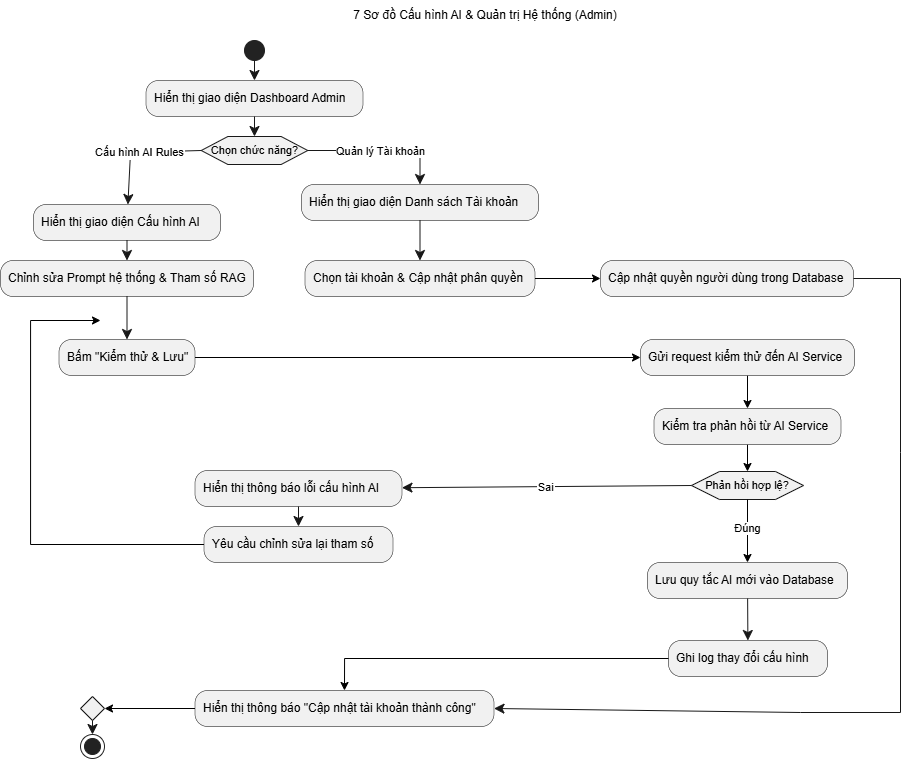
\includegraphics[width=0.85\textwidth]{Figures/Trang-3.drawio}
	\label{fig:luong_man_hinh_quantri}
\end{figure}

\clearpage % <-- Lệnh ngắt trang ĐẶT TẠI ĐÂY để ép toàn bộ BẢNG sang hẳn trang mới!

\renewcommand{\arraystretch}{1.25}
\begin{longtable}{|c|p{2.8cm}|p{4.2cm}|p{6.5cm}|}
	\hline
	\rowcolor{tableheader}
	\textbf{\#} & \textbf{Feature} & \textbf{Screen} & \textbf{Description} \\ \hline
	\endfirsthead
	1 & General & Trang chủ / Đăng nhập Quản trị & Cổng đăng nhập an toàn hạn chế truy cập cho ban quản trị học vụ. \\ \hline
	2 & Dashboard & Dashboard Quản trị viên Học vụ & Tổng quan chỉ số vận hành hệ thống, số lượng tài khoản hoạt động và khóa học mới. \\ \hline
	3 & User Management & Màn hình Quản lý Tài khoản \& Phân quyền User & Quản lý danh sách người dùng toàn hệ thống, cấp/thu hồi quyền truy cập theo vai trò. \\ \hline
	4 & User Management & Màn hình Chi tiết Hồ sơ \& Trạng thái Hoạt động & Xem lịch sử hoạt động, trạng thái tài khoản (Active/Locked) và thông tin cá nhân. \\ \hline
	5 & Academic Management & Màn hình Quản lý Chương trình Học \& Khung Đào tạo & Thiết lập chương trình đào tạo, danh mục môn học và sơ đồ cây kiến thức. \\ \hline
	6 & Course Management & Màn hình Quản lý Khóa học, Bài giảng \& Tài liệu & Quản lý chi tiết nội dung các khóa học, bài giảng video, tài liệu đính kèm trên hệ thống. \\ \hline
	7 & System Config & Màn hình Cấu hình Tham số \& Quy định Hệ thống & Cài đặt các tham số toàn hệ thống như thang điểm, quy định thời gian, thông báo. \\ \hline
	8 & Quality Control & Màn hình Kiểm duyệt Đề thi \& Nội dung Luyện tập & Giao diện duyệt các bộ đề thi, bài tập do giáo viên tải lên trước khi xuất bản. \\ \hline
	9 & Reporting & Màn hình Tổng hợp Báo cáo Học vụ \& Vận hành & Báo cáo chi tiết về tỷ lệ hoàn thành khóa học, hiệu suất giảng dạy và chất lượng đào tạo. \\ \hline
	10 & Data Export & Pop-up Xuất Dữ liệu \& Nhật ký Hệ thống (Logs) & Hộp thoại chọn định dạng và xuất file lưu trữ nhật ký hoạt động (system logs), báo cáo. \\ \hline
\end{longtable}

\begin{figure}[htbp]
	\centering
	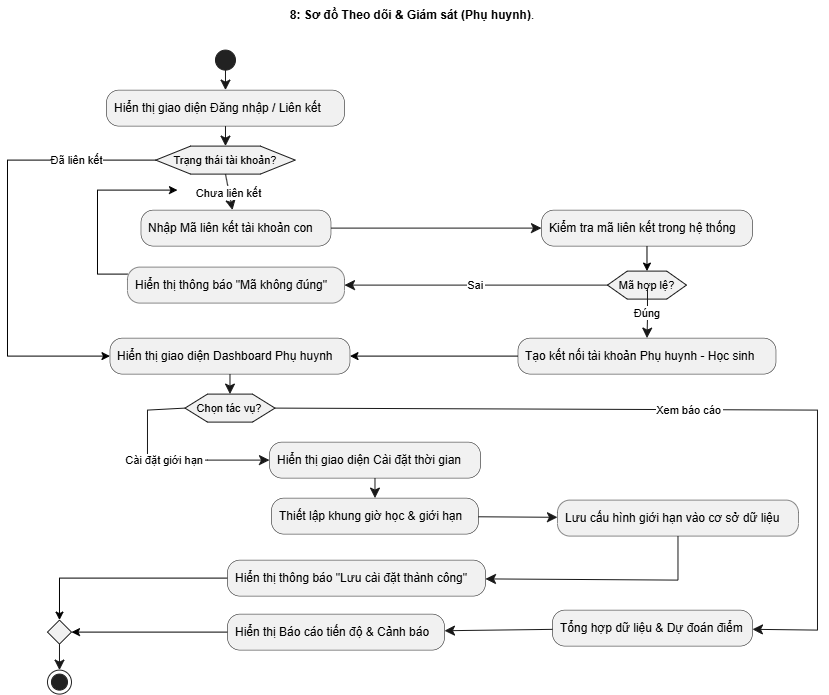
\includegraphics[width=0.85\textwidth]{Figures/Trang-4.drawio} % Đổi tên file ảnh tương ứng nếu cần
	\caption{Sơ đồ luồng màn hình hệ thống - Phụ huynh}
	\label{fig:luong_man_hinh_phuhuynh}
\end{figure}

\clearpage % Ngắt trang tại đây để toàn bộ bảng nằm trọn vẹn ở trang sau

\renewcommand{\arraystretch}{1.25}
\begin{longtable}{|c|p{2.8cm}|p{4.2cm}|p{6.5cm}|}
	\hline
	\rowcolor{tableheader}
	\textbf{\#} & \textbf{Feature} & \textbf{Screen} & \textbf{Description} \\ \hline
	\endfirsthead
	1 & General & Trang chủ / Đăng nhập Phụ huynh & Trang đăng nhập dành riêng cho phụ huynh theo dõi con em. \\ \hline
	2 & Dashboard & Dashboard Phụ huynh & Trung tâm điều khiển hiển thị tóm tắt tình hình học tập, lịch thi sắp tới của con. \\ \hline
	3 & Profile & Màn hình Chọn Hồ sơ Con / Học sinh & Cho phép chuyển đổi linh hoạt giữa các hồ sơ học sinh nếu phụ huynh có nhiều con theo học. \\ \hline
	4 & Progress Tracking & Màn hình Tổng quan Tiến độ Học tập của Con & Hiển thị phần trăm hoàn thành các khóa học, thời gian học tập trung bình mỗi ngày. \\ \hline
	5 & Academic Report & Màn hình Báo cáo Kết quả Thi \& Luyện tập Chi tiết & Bảng điểm chi tiết các bài kiểm tra, xếp hạng và kết quả các kỳ thi thử. \\ \hline
	6 & Attendance & Màn hình Theo dõi Lịch học \& Chuyên cần & Thời khóa biểu học tập, điểm danh các buổi học và lịch nộp bài tập. \\ \hline
	7 & Evaluation & Màn hình Xem Đánh giá từ Giáo viên \& Phân tích AI & Tổng hợp nhận xét trực tiếp từ giáo viên kết hợp báo cáo phân tích điểm mạnh/yếu từ AI. \\ \hline
	8 & Communication & Màn hình Khảo sát \& Trao đổi với Giáo viên & Kênh liên lạc trực tiếp giúp phụ huynh gửi tin nhắn, trao đổi với giáo viên chủ nhiệm/bộ môn. \\ \hline
\end{longtable}


\begin{figure}[htbp]
	\centering
	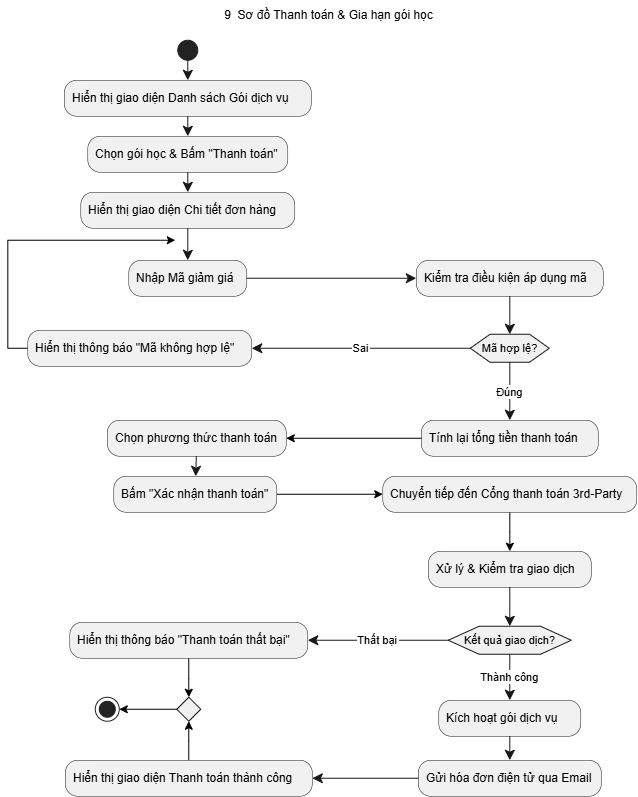
\includegraphics[width=0.85\textwidth]{Figures/Trang-5.drawio} % Đổi tên file ảnh tương ứng nếu cần
	\label{fig:luong_man_hinh_trang5}
\end{figure}

\clearpage % Ngắt trang tại đây để toàn bộ bảng nằm trọn vẹn ở trang sau

\renewcommand{\arraystretch}{1.25}
\begin{longtable}{|c|p{2.8cm}|p{4.2cm}|p{6.5cm}|}
	\hline
	\rowcolor{tableheader}
	\textbf{\#} & \textbf{Feature} & \textbf{Screen} & \textbf{Description} \\ \hline
	\endfirsthead
	1 & General & Trang chủ / Dashboard & Màn hình xuất phát cung cấp lối truy cập danh mục sản phẩm/khóa học. \\ \hline
	2 & Catalog & Màn hình Danh sách Gói học / Khóa học & Hiển thị danh sách các gói dịch vụ, khóa học lẻ, gói tài khoản VIP. \\ \hline
	3 & Package Detail & Màn hình Chi tiết Gói học \& Quyền lợi & Cung cấp thông tin đầy đủ về quyền lợi, thời hạn sử dụng và mức giá của gói học. \\ \hline
	4 & Checkout & Màn hình Đơn hàng \& Áp dụng Mã giảm giá & Màn hình xem tóm tắt đơn hàng, cho phép nhập mã voucher/Coupon ưu đãi. \\ \hline
	5 & Payment Setup & Màn hình Chọn Phương thức Thanh toán & Cho phép người dùng chọn kênh thanh toán (Ví điện tử, Chuyển khoản QR, Thẻ ATM/Visa). \\ \hline
	6 & Agreement & Màn hình Xác nhận Đơn hàng \& Điều khoản & Màn hình xem lại tổng số tiền thanh toán cuối cùng và đồng ý với điều khoản mua hàng. \\ \hline
	7 & Payment Gateway & Cổng Thanh toán Trung gian / Quét mã QR & Chuyển hướng sang giao diện cổng thanh toán (VNPay, Momo...) hoặc mã QR chuyển khoản. \\ \hline
	8 & Verification & Pop-up Xác thực Giao dịch (OTP / Mật khẩu) & Hộp thoại nhập mã OTP SMS/Soft OTP từ ngân hàng để hoàn tất giao dịch. \\ \hline
	9 & Confirmation & Màn hình Thông báo Thanh toán Thành công & Màn hình xác nhận giao dịch thành công kèm mã tham chiếu đơn hàng. \\ \hline
	10 & Invoice & Màn hình Chi tiết Hóa đơn Điện tử & Hiển thị và hỗ trợ tải xuống hóa đơn tài chính/hóa đơn bán hàng điện tử. \\ \hline
	11 & Transaction History & Màn hình Kích hoạt \& Lịch sử Giao dịch & Cập nhật trạng thái kích hoạt gói học trong tài khoản và lưu lịch sử giao dịch. \\ \hline
	12 & Course Access & Màn hình Vào Khóa học mới mua & Điều hướng người dùng bắt đầu trải nghiệm nội dung khóa học vừa đăng ký. \\ \hline
\end{longtable}



\begin{figure}[htbp]
	\centering
	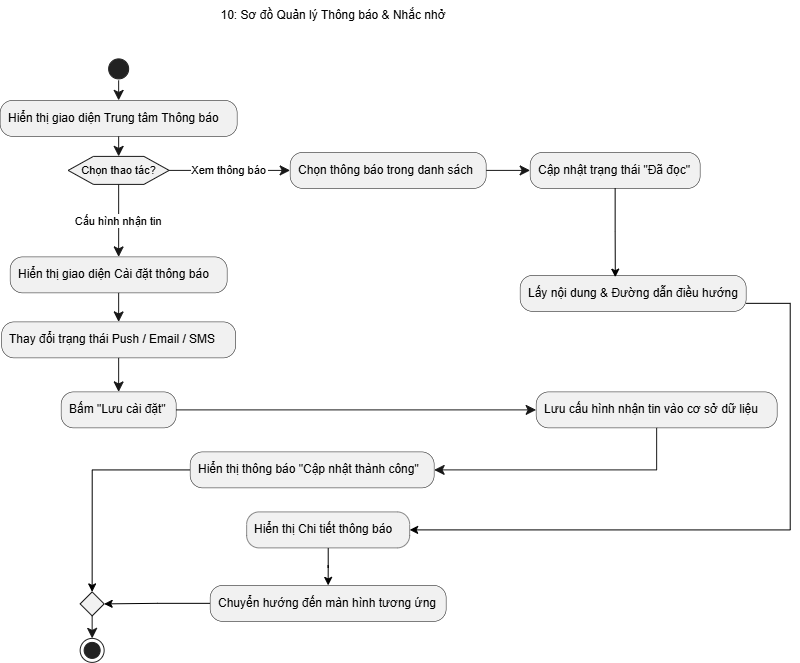
\includegraphics[width=0.85\textwidth]{Figures/Trang-6.drawio} % Đổi tên file ảnh tương ứng nếu cần
	\label{fig:luong_man_hinh_trang6}
\end{figure}

\clearpage % Ngắt trang tại đây để toàn bộ bảng nằm trọn vẹn ở trang sau

\renewcommand{\arraystretch}{1.25}
\begin{longtable}{|c|p{2.8cm}|p{4.2cm}|p{6.5cm}|}
	\hline
	\rowcolor{tableheader}
	\textbf{\#} & \textbf{Feature} & \textbf{Screen} & \textbf{Description} \\ \hline
	\endfirsthead
	1 & General & Trang chủ / Dashboard & Trang chính tích hợp biểu tượng quả chuông thông báo và lối tắt báo cáo. \\ \hline
	2 & Notifications & Trung tâm Thông báo (Notification Center) & Hộp thư chung hiển thị tất cả các thông báo mới gửi tới tài khoản. \\ \hline
	3 & Notification Categorization & Màn hình Phân loại Thông báo & Giao diện tab hỗ trợ lọc thông báo theo từng chủ đề: Lịch học, Điểm số, Hệ thống. \\ \hline
	4 & Notification Detail & Màn hình Chi tiết Thông báo & Hiển thị toàn bộ nội dung văn bản, hình ảnh hoặc tệp đính kèm của thông báo. \\ \hline
	5 & Navigation & Màn hình Điều hướng đến Tính năng Liên quan & Màn hình đích khi người dùng nhấn vào đường link liên kết trong thông báo. \\ \hline
	6 & Reporting Hub & Màn hình Trung tâm Báo cáo \& Thống kê Tổng hợp & Trang tổng quan báo cáo các chỉ số quan trọng toàn hệ thống hoặc cá nhân. \\ \hline
	7 & Filtering & Màn hình Thiết lập Bộ lọc Báo cáo & Cho phép thiết lập tiêu chí truy xuất dữ liệu: khoảng thời gian, học kỳ, lớp, môn học. \\ \hline
	8 & Data Visualization & Màn hình Hiển thị Biểu đồ \& Đồ thị Chi tiết & Trực quan hóa dữ liệu bằng biểu đồ cột, biểu đồ tròn, bảng số liệu so sánh. \\ \hline
	9 & Customization & Pop-up Tùy chỉnh Định dạng Báo cáo & Hộp thoại chọn các trường dữ liệu cần hiển thị trước khi tạo tệp báo cáo. \\ \hline
	10 & File Export & Pop-up Xuất File Báo cáo (PDF / Excel / CSV) & Hộp thoại xác nhận tải xuống file báo cáo theo định dạng tài liệu được chọn. \\ \hline
\end{longtable}